\chapter{Architectural Overview}
\label{chp:b3}

In this chapter, we introduce our proposed architecture of the mini driverless
car with its hardware and software components. We also present our simulation
environment, which was implemented to speed up the development and
verification processes.

\section{Hardware Configuration}

Autonomous cars are equipped with a powerful central computer, actuators and
many sensors such as IMU, Camera, and LIDAR. Our mini driverless car also has
the equivalent hardware components as shown in Figure
\ref{figure:hardware-configuration}. Details of these components are given in
Table \ref{table:hardware-configuration}.

\begin{figure}[h]
\centering
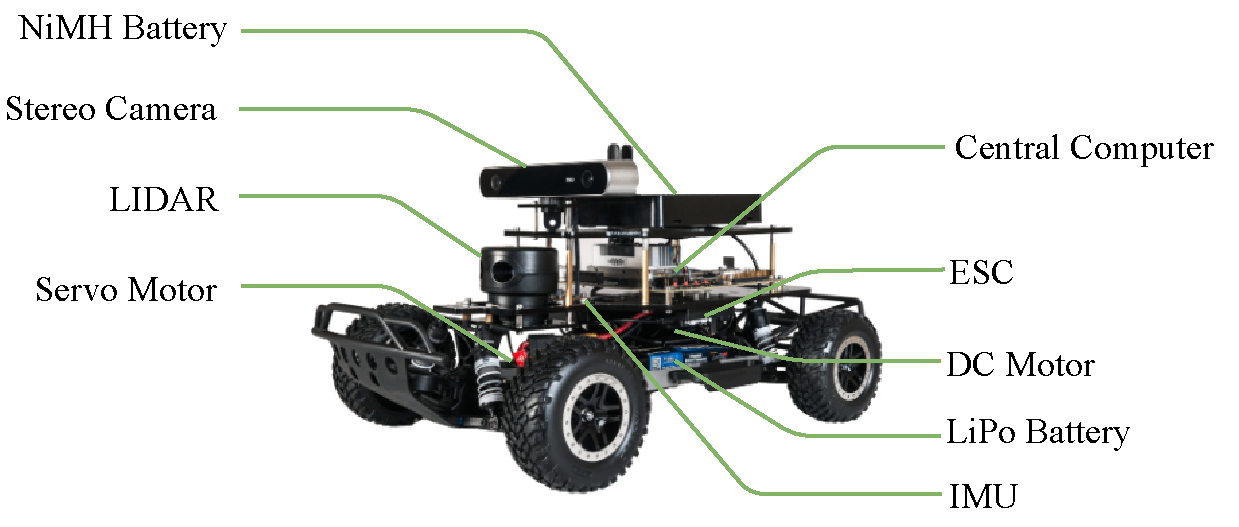
\includegraphics[width=.8\textwidth]{figures/hardware-configuration.pdf}
\caption{Hardware components on the mini driverless car.}
\label{figure:hardware-configuration}
\end{figure}

\begin{table}[h]
\caption{Mini driverless car hardware configuration details.}
\label{table:hardware-configuration}
\resizebox{\textwidth}{!}{\begin{tabular}{||c c||}
 \hline
 Component & Description \\ [0.5ex]
 \hline\hline
 Vehicle & TRAXXAS SLASH 4X4 PLATINUM EDITION \\ 
 \hline
 Central Computer & NVIDIA Jetson TX2 Developer Kit \\
 \hline
 Stereo Camera & Stereolabs ZED Camera \\
 \hline
 2D LIDAR & Scanse Sweep LIDAR \\
 \hline
 ESC & Vedder Electronic Speed Controller \\
 \hline
 IMU & SparkFun 9 DoF Razor IMU M0 \\
 \hline
 USB3.0 Hub & USB 3.0 7-Port Hub with 2 Charging Ports UH720 \\
 \hline
 Joystick & Logitech F710 Wireless Gamepad (940-000142) \\
 \hline
 LiPo Battery & 4200 mAh 7,4V 25C \\
 \hline
 NiMH Battery & MARC Power Lite 3400mAh 16V and 12V outputs \\ [1ex]
 \hline
\end{tabular}}
\end{table}

The central computer runs various sophisticated algorithms to fuse raw data
from sensors to achieve situational awareness, select the best possible action
accordingly, and finally send speed and steering angle commands to the ESC.  in
order to execute the action. The ESC generates necessary electronic signals
from the commands and feeds them to servo and DC motors to control steering
angle and speed, respectively. We replace the stock ESC that ships with the
vehicle with a different speed controller known as VESC, an open source ESC,
since it is highly configurable and thus supports full control at lower speeds
\cite{cite2}. The hardware setup also provides a joystick control in order to
acquire dataset from a human driver and take over the control during the
autonomous drive in case of an emergency. We use two different batteries to
power the vehicle.  While NiMH battery powers the central computer and sensors
through the USB 3.0 Hub, LiPo battery supplies current to the actuators as they
need a more consistent power source in both quality and quantity.

\section{Software Architecture}

We use Robot Operating System (ROS) \cite{cite3} to implement our architecture.
ROS defines notion of nodes and allows nodes to communicate through
publish/subscribe and reply/request mechanisms. Similar to \cite{cite1}, we
also rely on publish/subscribe mechanism for the data flow between our nodes.
Nodes subscribe to the message streams from other nodes. The result of the
computation of a node is then published to the other nodes. This asyncrononous
messaging alows the software to act as a data processing pipeline. The
architecture is roughly grouped into four modules.

\begin{itemize}
    \item \textbf{sensor interface --} The sensor interface reads raw data from
        individual sensors, converts them to meaningful engineering data, then
        feeds them to the other modules.
    \item \textbf{scene interpretation --} The scene interpretation module
        makes sense of the the the environment by finding traffic lanes,
        detecting obstacles, and classifying the traffic signs. Once the
        objects of interests are detected and classified, the module also
        locates the these objects in the real world coordinates with respect to
        car's body frame. Then it decides on a high-level behavior that best
        fits to its current perception of the environment such as keeping a
        lane or stopping on a red light.
    \item \textbf{navigation --} The navigation module first takes the
        kinematic constraints, traffic rules, and nearby obstacles into account
        and generates an optimal trajectory to realize the high-level behavior.
        Then it computes steering angle and speed values in order to follow the
        optimal trajectory as close as possible.
    \item \textbf{actuator --} A pre-configured firmware in the VESC converts
        steering and speed commands into electronic signals to drive the
        motors.
\end{itemize}

Figure \ref{figure:software-architecture} illustrates the overall data flow in
the software modules. Out of these modules, nodes in sensor interface and
actuator modules are already provided as ROS packages. They are not implemented
but configured within the scope of this thesis.

\begin{figure}[h]
\centering
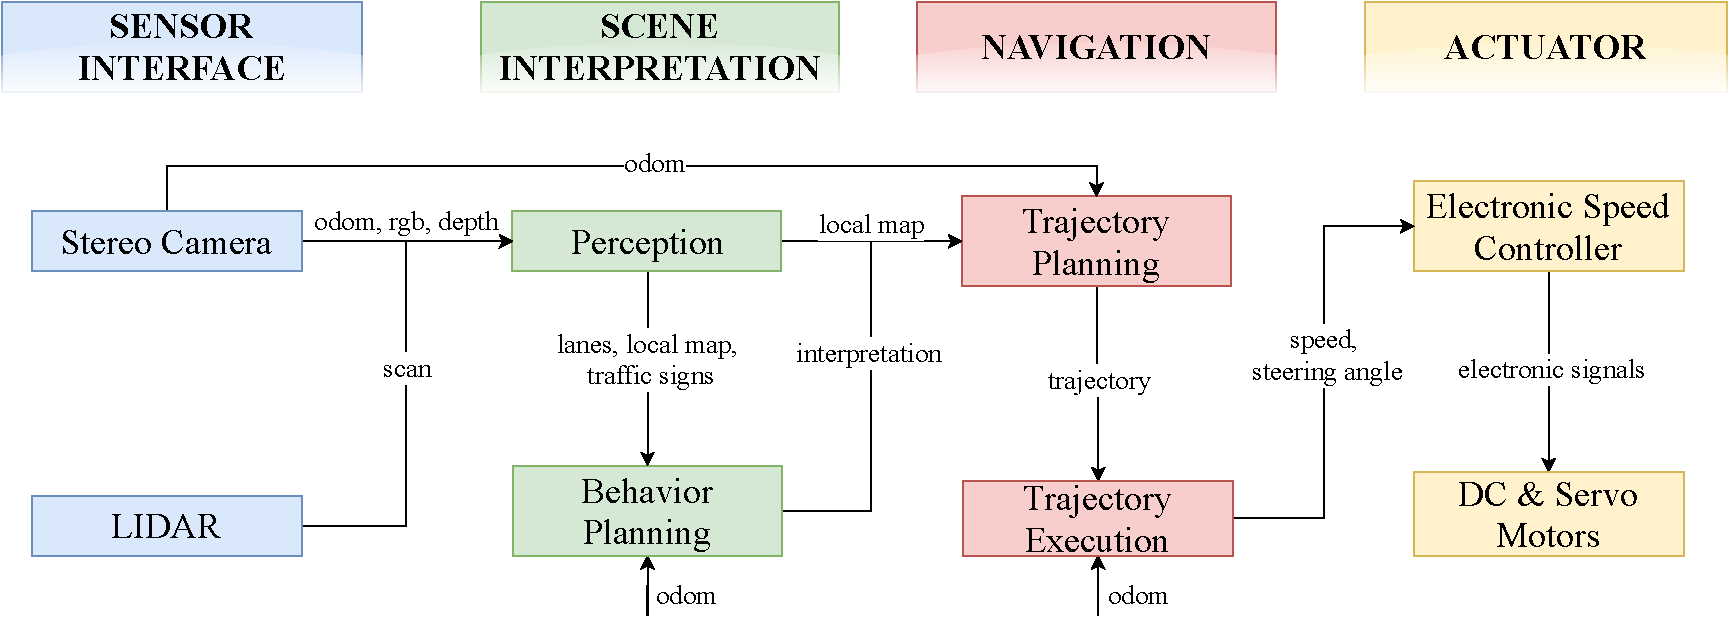
\includegraphics[width=.9\textwidth]{figures/software-architecture.pdf}
\caption{Software architecture overview.}
\label{figure:software-architecture}
\end{figure}

Zed camera node is configured to publish visual odometry, RGB, and depth topics
at the rate of 15 Hz. Message types flow through this topics are well-defined
in ROS. An odometry message contains position, orientation, linear and angular
velocities with respect to the starting point, i.e. with respect to the
odometry frame. RGB image message is a rectified color image from the left zed
camera, which is used for image segmentation and classification. Because zed
camera features stereo images, it can also publish a depth image, which is used
to locate the traffic signs with respect to the body frame.

LIDAR node is configured to provide scan data to the costmap nodes in the scene
interpretation module at 5 Hz rotational speed. The costmap nodes then
publishes local occupancy grid maps that indicate nearby objects. Scene
interpretation maintains two local maps in different sizes. The small map is
used in navigation module for collision avoidance.  The larger map is
internally used by the scene interpretation module for behavior planning to
guide the trajectory planner before the navigation module observe the
obstacles.

Behavior planner component decides if the car should stop or in which speed
range it should move, whether it should track the lanes or follow a predefined
path. At the end, the behavior planner captures the current desired
behavior in an interpretation message and publishes to the trajectory planner.

Trajectory planner subscribes to the odometry, 3x3 local map, and
interpretation topics so as to find a collision-free, kinematically feasible,
smooth, and optimal trajectory. The trajectory message contains waypoint
locations in the odometry frame and a recommended speed for each waypoint.

Finally, given the odometry and optimal trajectory, the trajectory execution
node computes steering angles to closely follow the optimal trajectory and
publishes the recommended speed and steering commands to the actuator module.

\section{Simulation Environment}

It is not always practical to try new ideas on the target platform for several
reasons. First, it is too risky to run an updated version of software in the
target platform as it would crash into an obstacle. Second, the batteries have
certain life time and we do not want to drain them for each immature update to
the code base. Third, deploying ad testing the software on the target is time
consuming. The last but not least, because running the software on the target
requires a large enough spacial area with various traffic signs, lanes, a
bridge and many other urban conditions, which we could barely afford a few, we
had no better option than creating a simulated environment.

We used Gazebo to model our simulation world and robot car. Figure
\ref{figure:simulation-environment} shows the simulated urban area. It
simulates every case in OpenZeka MARC 2019 except that we have to manually
replace red and green lights, and manually remove the pedestrian from the
scene.

\begin{figure}[h]
  \centering
  \begin{subfigure}[b]{0.4\linewidth}
      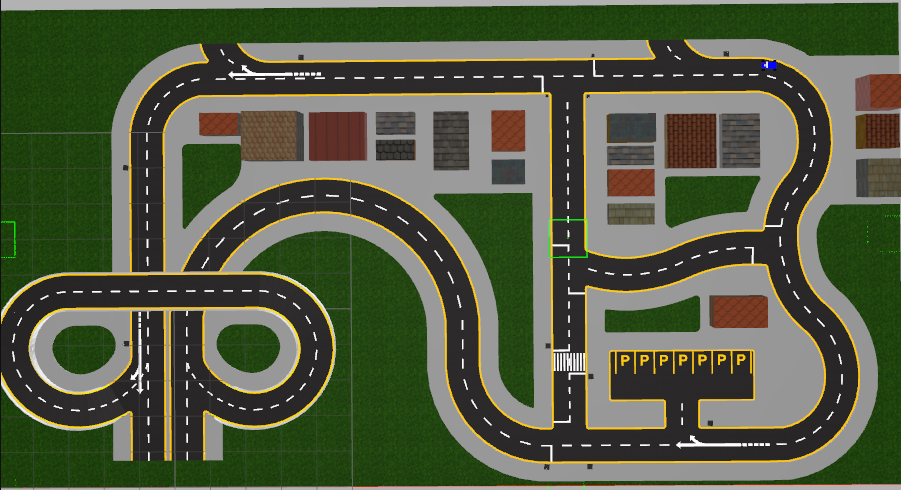
\includegraphics[width=\linewidth]{figures/simulation-environment1.png}
    \caption{}
  \end{subfigure}
  \begin{subfigure}[b]{0.4\linewidth}
      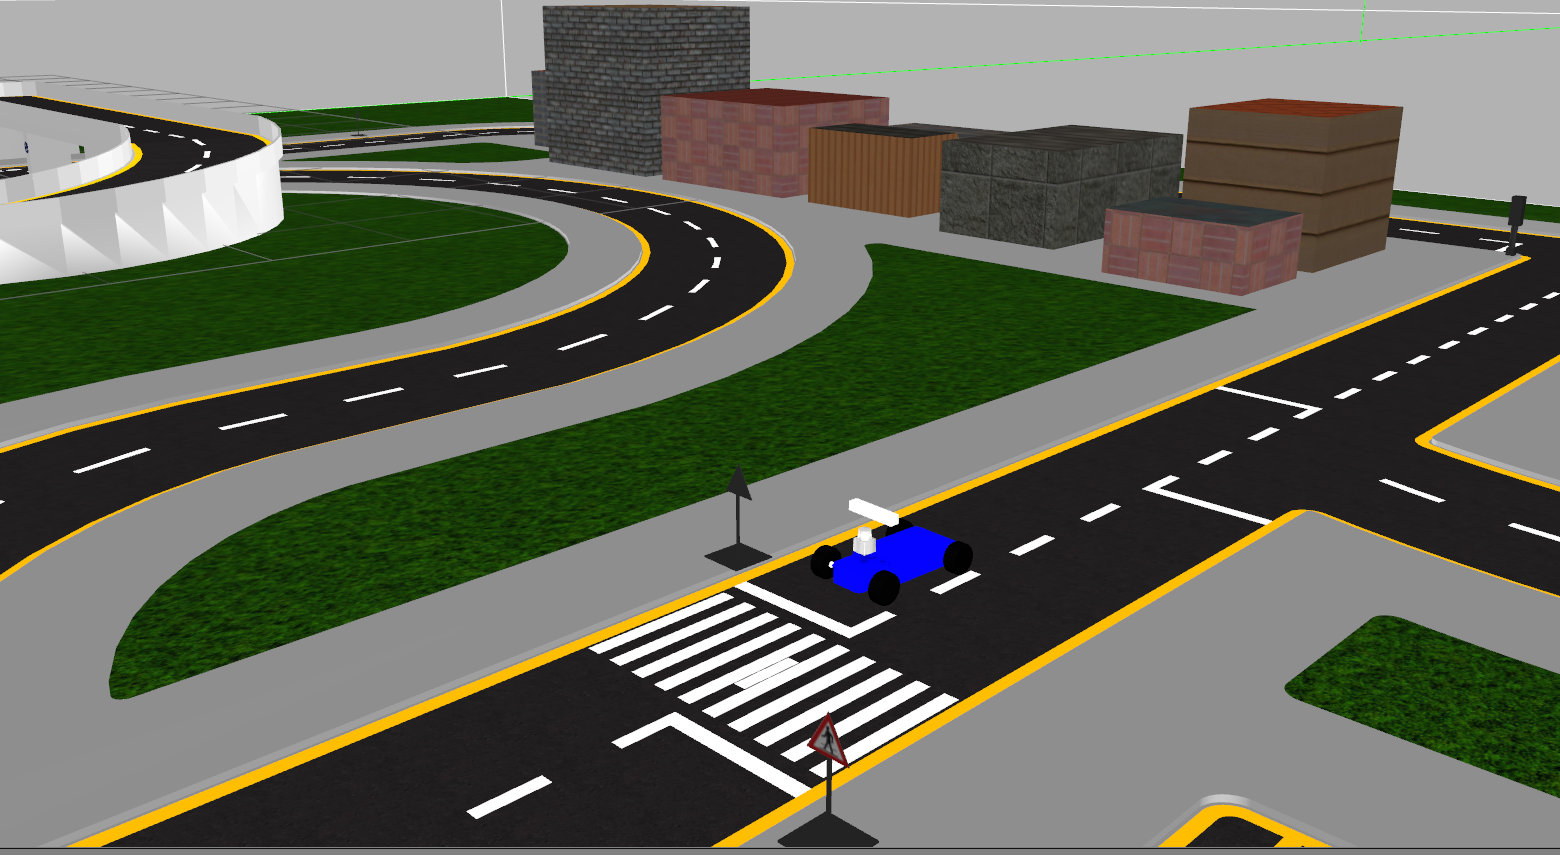
\includegraphics[width=\linewidth]{figures/simulation-environment2.png}
    \caption{}
  \end{subfigure}
  \caption{(a) Gazebo simulation environment top view. (b) The car, traffic
  signs, and the bridge in the simulation environment.}
  \label{figure:simulation-environment}
\end{figure}

Simulated sensors were also carefully tuned to reflect actual sensor behaviors,
but still actual camera images look blurrier. Moreover, we did not simulate the
changing lighting conditions and vibrations from the actuators. Figure
\ref{figure:camera-view} gives the actual and simulated camera views for
comparison.

\begin{figure}[h]
  \centering
  \begin{subfigure}[b]{0.4\linewidth}
      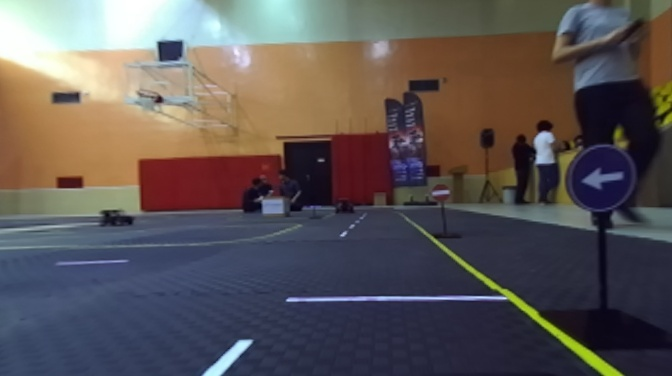
\includegraphics[width=\linewidth]{figures/actual-camera-view.jpg}
    \caption{}
  \end{subfigure}
  \begin{subfigure}[b]{0.4\linewidth}
      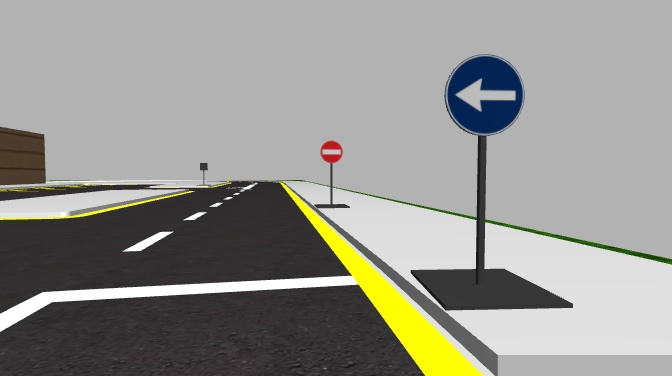
\includegraphics[width=\linewidth]{figures/simulated-camera-view.jpg}
    \caption{}
  \end{subfigure}
  \caption{(a) Actual camera view. (b) Simulated camera view.}
  \label{figure:camera-view}
\end{figure}

Despite all the peculiarities of the simulation environment, it made it
possible to quickly collect datasets without needing any additional hardware,
not even a joystick as it supports keyboard commands. We trained our
segmentation and classification models on those datasets and tested in the
simulation environment. We also developed our trajectory planning and control
algorithms in the simulation, which drastically reduced the risk of damaging
any equipment. On the whole, the simulation did not replace the real world, but
rather served as a flexible testbed.
